\documentclass[letterpaper,10pt,twocolumn]{../aspe}

% ===>>> Replace the paper title with yours.

\title{ASPE Manuscript Template}

% ===>>> Replace the author list with yours.
%        Use superscript numbers ($^number$) to identify the correct
%        institution, if more than one is being listed below.

\author{Jane Q. Author$^1$, Frank A. Author$^1$, and Javier J. Author$^2$}

% ===>>> Replace affiliations with yours.  Use leading superscript
%        numbers to identify institutions as they are referred to
%        by the superscript numbers in the list of authors.

\affiliations{$^1$Department or Division\\
Company or University\\
City, State, or Province, Country \\
$^2$Department or Division\\
Company or University\\
City, State or Province, Country}

%   The following packages provide support for figure and math
%   formula and symbol display, leave them in anyway.
%   They are part of LaTeX and should therefore be always available.

\usepackage{graphicx}
\usepackage{amsmath}
\usepackage{amssymb}

%   Limit separation of text from tables and figures in the middle
%   to a single line's worth.

\intextsep=\lineskip


\begin{document}
\maketitle
\section*{Instructions}   % Note the asterisk.
This document provides instructions for preparing a manuscript for the proceedings of an {ASPE} conference. You may want to use the source file of this template directly to prepare
your paper.  The desired formatting is accomplished basically by using a class file
``ASPE\_ExtendedAbstract.cls'' which is a variation of the standard ``article.cls'' file.  It is invoked in the first line of your document source
file:
{\topsep=0pt
\begin{flushleft}
    \hspace*{3mm}$\backslash$documentclass[letterpaper,10pt,\linebreak
            \hspace*{6mm}twocolumn]\{ASPE\_ExtendedAbstract\}
\end{flushleft}
}

The assumed physical paper size is 8.5'' $\times$ 11'' (216 by 279 mm \underline{US letter size}) with a 1'' (25.4 mm) margin all around.

Your paper should begin one line below the author list.  The text of your
paper should be single spaced, 10-point Helvetica-like font using justified
alignment in a two column format. Each column should be 3'' (76.2 mm) wide
with a 0.5'' (12.7 mm) spacing between columns. Spacing between paragraphs
should be one line.

For the Annual Meeting, papers should be 4--6 pages long, including tables and figures. For other meetings, a different limit may be posted on the ASPE website.
\emph{Do not use page numbers, headers, or footers within the manuscript.}

Footnotes may be included, if required.\cite{Lamport1986} These can be
written as follows in the main text:\footnote{This is a footnote
    referred to in the regular text.  Refer to Lamport's
    book \cite{Lamport1986} on how to do this inside, e.g., a table or a
    caption.}
{\topsep=0pt
    \begin{flushleft}
        \hspace*{3mm}$\backslash$footnote\{This is a footnote referred to\linebreak
        \hspace*{6mm}in the regular text.  Refer to Lamport's\linebreak
        \hspace*{6mm}book $\backslash$cite\{Lamport1986\} on how to do\linebreak
        \hspace*{6mm}this inside, e.g., a table or a caption.\}
    \end{flushleft}
}
Most formatting requirements described throughout this document (including
paper size, two-column format, font, font size, spacings, margins, no
page numbers, headers nor footers) are automatically taken care of by the
class file and the ``$\backslash$documentclass'' command.

\section*{PAPER TITLE AND AUTHOR(S)}
The title and author information, plus a few other LaTeX commands, appear between the opening ``$\backslash$documentclass'' and the ``$\backslash$begin\{document\}''
commands.  The title of your paper should start 1'' (25.4 mm) from the top
of the page and be 14-point bold, Helvetica font in all capital letters.
The title should be centered on the page. One line space should separate
the title from the author listing(s).  The command

\hspace*{3mm}$\backslash$title\{ASPE Manuscript Template\}

will accomplish all of this.  Just substitute your own title.

Each author name should consist of first name, middle initial, and last
(family) name. It should be 12-point Helvetica bold, upper and lower case
letters, centered under the title. All authors should be listed on the same
line with their affiliations identified by numeric superscripts at the end
of the name.  (In the case of a single author, do not use a superscript.)
Author affiliation(s) should consist of the following, as applicable:
\begin{list}{$\bullet$}{\labelsep=0.1in\parsep=0pt\parskip=0pt}
    \item department or division name
    \item company or university
    \item city, state or province, and country.
\end{list}
All author affiliation information should be 12-point Helvetica bold, upper
and lower case letters, centered under the name. For more than two author
affiliations, they may be listed in double columns.

\section*{Text Heading \#1}
The primary section or text heading should be 10-point Helvetica bold, all
capital letters, flush left with the margin. If the heading is more than
one line, the following lines should also be flush left. The spacing to the
next heading should be one line.  All of this is accomplished with the
command (note the asterisk):

\hspace*{3mm}$\backslash$section*\{Text Heading $\backslash$\#1\}

\subsection*{Text Heading \#2}
The first sub-heading should be 10-point Helvetica bold, upper and lower
case letters, and underlined. The heading is flush left, and the spacing
to the next heading is one line.  All of this is accomplished with the
command (note the asterisk):

\hspace*{3mm}$\backslash$subsection*\{Text Heading $\backslash$\#2\}

\subsubsection*{Text Heading \#3}
The third level of heading should be 10-point Helvetica bold, upper and
lower case letters, and italicized. The heading is flush left, and the
spacing to the next heading is one line.  All of this is accomplished
with the command (note the asterisk):

\hspace*{3mm}$\backslash$subsubsection*\{Text Heading $\backslash$\#3\}

\subsection*{Another subsection}\vspace{2\parskip}
\subsubsection*{Subsubsection leading off in a subsection}
Whenever a lower section level header follows immediately on a higher
one, i.e., no regular test in between, a command
``$\backslash$vspace\{2$\backslash$parskip\}`` needs to be inserted
between the two (sub)section header commands.
\section*{FIGURES, TABLES, AND PHOTOS}
Figures, tables and photos may be in color, but note that the printed
proceedings will be in black and white, so multiple data sets in graphs
should be clearly identified with this in mind.

Text within the figures should have a font size of not less than 8-point.
Photographs should be scanned at 144 dots per inch (dpi) and inserted as
graphic objects into the document. With LaTeX, the ``graphicx'' package
included before the ``$\backslash$begin\{document\}'' command is used to
handle the
graphics.  Figures and tables should be numerically labeled consecutively;
in LaTeX, the ``$\backslash$caption'' command inside the figure and table
definitions takes care of the desired numbering.  Inserting a
``$\backslash$label\{tableone\}'' command (with ``tableone'' being just an
example for a label name) inside the caption provides you with a means to
refer to the figure or table number with the ``$\backslash$ref'' command as in
``Table $\backslash$ref\{tableone\}'', which gives: ``Table \ref{tableone}''.
Note that whenever you add a new reference (figure, table or bibliographic),
or reorder their appearance, you have to run your LaTeX processor twice
to make the output appear correctly.

An example each for a table and a figure with captions are provided below,
in two-column format.
If necessary, tables and figures may be inserted using a single column
format.

The table identification (e.g., TABLE \ref{tableone}) should be 10-point
Helvetica, all capitals, italicized, and end with a period. It should be
placed above the table.
The table caption should follow the table identification and should be
10-point Helvetica font, upper and lower case letters, italicized, and
justified.  The placement is accomplished by putting the
``$\backslash$caption'' command in the table structure before the body of
the table.
    {\topsep=0pt
        \begin{flushleft}
            \hspace*{3mm}$\backslash$begin\{table\}[htb]\linebreak
            \hspace*{3mm}$\backslash$caption\{$\backslash$label\{tableone\}\{This
            is\linebreak
            \hspace*{6mm} the sample table caption.\}\}\linebreak
            \hspace*{3mm}$\backslash$vspace\{10pt\}\linebreak
            \hspace*{3mm}$\backslash$begin\{tabular\}[]\{|c|c|c|\}\linebreak
            \hspace*{3mm}$\backslash$hline\linebreak
            \hspace*{3mm}Index \& Value 1 \& Value 2 $\backslash\backslash$
            $\backslash$hline\linebreak
            \hspace*{3mm}1 \& 0.1 \& 0.6 $\backslash\backslash$\linebreak
            \hspace*{3mm}2 \& 0.5 \& 1.5 $\backslash\backslash$\linebreak
            \hspace*{3mm}3 \& 1.2 \& 3.5 $\backslash\backslash$ $\backslash$hline
            \linebreak
            \hspace*{3mm}$\backslash$end\{tabular\}\linebreak
            \hspace*{3mm}$\backslash$end\{table\}
        \end{flushleft}
    }
The ``$\backslash$vspace'' command places a vertical space of 10 pt
between the caption and the body of the table.
The letters h, t and b in the square brackets indicate that LaTeX will
first try to place the table within the text where it is defined (``h''
for ``here'').  If that runs afoul of a column break, it will try to place
it at the top (``t'') or bottom (``b'') of a column.
The ampersants ``\&'' separate columns, and the double backslashes separate
rows.  The ``$\backslash$hline'' commands and the bars and ``c''-s in the
``$\backslash$begin\{tabular\}'' command create the outlines of the table and the
centering (``c'') of the columns.  For more details about how to control the
appearance of the table see Lamport's book.\cite{Lamport1986}
Here is the resulting table:
\begin{table}[htb]
    \caption{\label{tableone}{This is the sample table caption.}}
    \vspace{10pt}
    \begin{tabular}[]{|c|c|c|}
        \hline
        Index & Value 1 & Value 2 \\ \hline
        1     & 0.1     & 0.6     \\
        2     & 0.5     & 1.5     \\
        3     & 1.2     & 3.5     \\ \hline
    \end{tabular}
\end{table}

Figures are handled quite similarly to tables.  In place of the body of the
table, a graphics file is referenced by the ``$\backslash$includegraphics'' command,
and the caption is placed below the image (Figure \ref{samplefigure})
rather than above.
\begin{figure}[htb]
    \begin{center}
        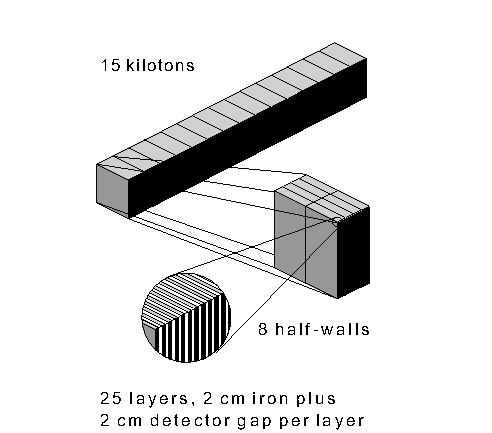
\includegraphics[width=3in,keepaspectratio=true]{node.pdf}
    \end{center}
    \caption{\label{samplefigure} The figure identification (e.g., FIGURE 1)
        should be 10-point Helvetica, all capitals, italicized and end with a
        period. It should be placed below the figure. The figure caption should
        follow the figure identification and should be 10-point Helvetica font,
        upper and lower case letters, italicized, and justified.}
\end{figure}

\section*{Acknowledgments}
Please make sure to acknowledge the contributions of people who are not
listed as authors, and of the support by institutions and funding agencies.

\section*{The last section: References}
References should be set in the same typeface as the text. They should appear
at the end of your paper and be arranged in order of appearance in the
text. Within the text, they should be numerically identified using closed
brackets. For example, to identify the first reference, use the
format [1], i.e., numbers in square brackets.
With LaTeX, you write that as

\hspace*{3mm}$\backslash$cite\{refname\}

The parameter ``refname'' reappears in the list of references at the
end of your paper.  LaTeX takes care of the sequential numbering.
The format follows the ``Vancouver'' numbered style, described at

http://www.icmje.org

The section on references can also be found at

http://www.nlm.nih.gov/bsd/\linebreak
\hspace*{1.2in}uniform\_requirements.html

%This format is also used for the Precision Engineering journal.

An easy, manual way to create the actual list of references is to use the
``$\backslash$bibitem'' command as follows:
{\topsep=0pt
\begin{flushleft}
    \hspace*{3mm}$\backslash$begin\{thebibliography\}\{23\}\linebreak
    \hspace*{3mm}$\backslash$bibitem\{Lamport1986\}Lamport, L.\linebreak
    \hspace*{6mm} LaTeX - A Document Preparation System,\linebreak
    \hspace*{6mm} Reading, MA, USA: Addison-Wesley\linebreak
    \hspace*{6mm} Publishing Company; 1986.\linebreak
    \hspace*{3mm}$\backslash$bibitem\{Lindeke1991\}Lindeke R.,\linebreak
    \hspace*{6mm} Schoenig F Jr, Khan A, Haddad J.\linebreak
    \hspace*{6mm} Machining of \$$\backslash$alpha,$\backslash$beta\$-Titanium
        \linebreak
        \hspace*{6mm} with Ultra-High Pressure Through the Insert\linebreak
        \hspace*{6mm} Lubrication/Cooling. Transactions of the\linebreak
        \hspace*{6mm} North American Manufacturing Research\linebreak
        \hspace*{6mm} Institution of SME. 1991; 19: 154-161.\linebreak
        \hspace*{3mm}$\backslash$bibitem\{Trigger1951\}Trigger K,Chao B.\linebreak
        \hspace*{6mm} An Analytical Evaluation of Metal Cutting\linebreak
        \hspace*{6mm} Temperatures. ASME Transactions, Journal\linebreak
        \hspace*{6mm} of Engineering for Industry. 1951; 73:\linebreak
        \hspace*{6mm} 57-68.\linebreak
        \hspace*{3mm}$\backslash$bibitem\{Ulsoy1989\}Ulsoy A, DeVries W.\linebreak
        \hspace*{6mm} Microcomputer Applications in\linebreak
        \hspace*{6mm} Manufacturing.  John Wiley and\linebreak
        \hspace*{6mm} Sons, Inc.  New York: 1989.\linebreak
        \hspace*{3mm}$\backslash$end\{thebibliography\}
\end{flushleft}
}
The parameter ``\{23\}'' indicates the widest space that needs to be
reserved in the list of references for the reference numbers
as 2 fairly wide digits (``1'' is narrower
than all the others).  The resulting list of references appears at the
end of this template paper.

The drawback of this manual method is that in order to
have the reference numbers appear in the running text in sequential order,
you have to know in which sequence they are used in the paper and sort the
``$\backslash$bibitem'' commands into that specific order.  For working with a
BIBTeX database, see the correspondign version of this document and
Lamport's book.\cite{Lamport1986}

\section*{PORTABLE DOCUMENT FORMAT (PDF)}
Please submit your abstract as an Adobe Acrobat (PDF) file to be included
in the electronic and bound conference proceedings.  This means that you
must make an Acrobat version after you have created the manuscript using
your favorite word processing software, and you
\underline{must} embed all fonts used in the PDF file.

    {\bf Protected Documents}:  It is very important that you not send documents that are password protected or otherwise secured.  The publisher must be able to open the PDF files to add page and volume numbers. ``Read or Print Only'' documents cannot be included in the Proceedings.

\section*{PAPER SUBMISSION}
Please follow the directions on the website at \emph{aspe.net} for links to the online submission portal, and details of conference submission deadlines.

\section*{QUESTIONS}
Please direct any questions to the ASPE Executive Director.
\begin{list}{}{\parsep=0pt\parskip=0pt}
    \item Telephone: (919) 839-8444
    \item Email: executive@aspe.net
\end{list}
Note that the Executive Director may forward specific questions to qualified
volunteers within the ASPE.

\begin{thebibliography}{23.}
    \bibitem{Lamport1986}Lamport L. LaTeX - A Document Preparation System.
    Reading, Massachusetts, USA: Addison-Wesley Publishing Company; 1986.
    \bibitem{Lindeke1991}Lindeke R, Schoenig F Jr, Khan A, Haddad J.
    Machining of $\alpha,\beta$-Titanium with Ultra-High Pressure Through
    the Insert Lubrication/Cooling. Transactions of the North American
    Manufacturing Research Institution of SME. 1991; 19: 154-161.
    \bibitem{Trigger1951}Trigger K, Chao B.  An Analytical
    Evaluation of Metal Cutting Temperatures. ASME Transactions, Journal of
    Engineering for Industry. 1951; 73: 57-68.
    \bibitem{Ulsoy1989}Ulsoy A, DeVries W.
    Microcomputer Applications in Manufacturing.
    John Wiley and Sons, Inc.  New York: 1989.
\end{thebibliography}

\end{document}
